\chapter{Hero Run Data Analysis} 
\label{chapter5}

The fully scaled version of the Early Earth simulation, referred to as the HiPerGator Hero Run, represents the most extensive molecular dynamics (MD) simulation ever conducted with a machine-learned interatomic potential. This ambitious project was a collaboration between the HiPerGator research computing team, NVIDIA, and the Roitberg group, leveraging cutting-edge GPU technology and state-of-the-art neural network potentials to model prebiotic chemistry on an unprecedented scale.

The Hero Run was conducted over six days, utilizing thousands of GPUs across the entire HiPerGator supercomputer to simulate 4.5 nanoseconds of reactive molecular dynamics. The temperature profile of the simulation was carefully designed to mimic potential prebiotic reaction conditions, incorporating both high-temperature chemistry and cooling cycles to explore the formation and stability of complex molecular species. The timeline of the simulation included: 0.05 ns heating from 0 K to 300 K, 0.2 ns heating from 300 K to 2500 K, 4.0 ns at 2500 K allowing extensive bond rearrangement, finally 0.25 ns cooling back to 300 K enabling the analysis of stable reaction products.
This temperature cycle was selected based on experimental and computational studies of high-energy impact chemistry, where transient high temperatures enable chemical bond rearrangement, followed by rapid cooling to capture stable reaction products.

The simulation encompassed a massive 22.8 million atoms, making it one of the largest reactive MD simulations ever conducted. ANI-1xnr, a machine-learned interatomic potential, provided near-quantum accuracy while maintaining the efficiency required to run such an extensive system. However, running a simulation at this scale posed significant computational challenges.
The next sections detail the strategies developed to process, analyze, and extract meaningful insights from this unprecedented dataset, including graph-based molecular identification, GPU-accelerated trajectory filtering, and large-scale clustering techniques.

\section{Molfind}
\label{sec:molfind}

MolFind is a protocol written in Python with RAPIDS 
%[cite] 
GPU-accelerated libraries which operates by translating each simulation snapshot into a graph data structure on the GPU, where atoms are represented as graph vertices and pairwise interactions (e.g., bonds or neighbor connections) become edges. To construct this graph, the tool leverages GPU-based neighbor-list building, using either cell-list or cutoff methods, and then uses the cuGraph library to create and store the adjacency information in GPU memory. Once the atom-level graph is established, MolFind performs connected-component searches to identify sets of atoms that form discrete molecular fragments, thus mapping the complex MD snapshot into discrete graph partitions. After extracting these connected subgraphs, it computes a flattened chemical formula for each fragment by collecting and sorting atomic species, which helps identify the basic stoichiometry. To capture structural details beyond mere composition, MolFind also assembles a “signature” string that encodes the internal connectivity—each bond is represented in a standardized format (e.g., sorted alphabetically as “C-H”) and aggregated to form a reproducible fingerprint. This combination of stoichiometric and connectivity descriptors ensures that fragments with identical compositions but different bond arrangements (e.g., isomers) can be distinguished. Finally, if desired, MolFind compares each fragment’s subgraph to a prebuilt reference database of molecular graphs. These comparisons involve GPU-accelerated manipulations and, where necessary, a final CPU-based isomorphism check with the NetworkX library 
%[cite] 
to verify exact structural matches. By keeping the core graph-building and connected-component search on the GPU, MolFind can scale to millions of atoms, enabling users to sweep through extended trajectories, track how molecular species evolve over time, and detect rare or unexpected products in large reactive systems.

\subsection{GraphMatcher}
\label{subsec:molfind_graphmatcher}

The GraphMatcher step in MolFind is responsible for determining whether a newly discovered fragment in a simulation matches any of the reference molecules in a provided database. After extracting the topology of each fragment as a graph (where nodes are atoms and edges represent bonds), MolFind adorns edges and nodes with additional labels—nodes store the atomic element, and edges store the bonded element pair (e.g., $\text{C–N}$, $\text{H–O}$). The tool then constructs an equivalent “reference graph” for each known molecule in the database, storing the same node and edge attributes. The matching procedure uses NetworkX’s GraphMatcher, specifically a categorical node match and categorical edge match strategy, to ensure that corresponding atoms and bonds must have the same chemical identity for the two subgraphs to be considered isomorphic. If the subgraph is determined to be isomorphic to a reference, MolFind assigns the corresponding label (e.g., “alanine” or “glycine”) to the fragment. 

In early development, some structures were mistakenly identified as alanine (Figure \ref{fig:mismatched_alanine}), underscoring the importance of carefully specifying node and edge attributes and verifying the molecular configuration.

\begin{flushleft}
\begin{multiFigure}
    \addFigure{0.5}{Images/early_earth/remakenot_alanine.png}
    \addFigure{0.5}{Images/early_earth/remakenot_alanine_silhouette.png}
\captionof{figure}[Mismatched structure of alanine]{
(A) Structure identified as alanine; 
(B) how the GraphMatcher was interpreting this structure, which makes it appear to be an alanine molecule.}
\label{fig:mismatched_alanine}
\end{multiFigure}
\end{flushleft}

In particular, if nodes were not distinctly labeled by their atomic species, or edges were not checked for precise element pairs, the GraphMatcher could falsely declare an isomorphism, conflating dissimilar fragments. By refining the graph-building procedure—ensuring that each node had the correct element label and each edge the correct pair of elements—MolFind began to more accurately match molecules in large-scale simulations. This adjustment led to corrected counts for species originally overestimated due to misidentification (Figure \ref{fig:graph_matching}). In practice, once node and edge attributes are rigorously assigned, the GraphMatcher becomes a powerful method for confirming the presence of specific molecules within highly complex molecular dynamics trajectories.

\begin{figure}[!ht]
    \centering
    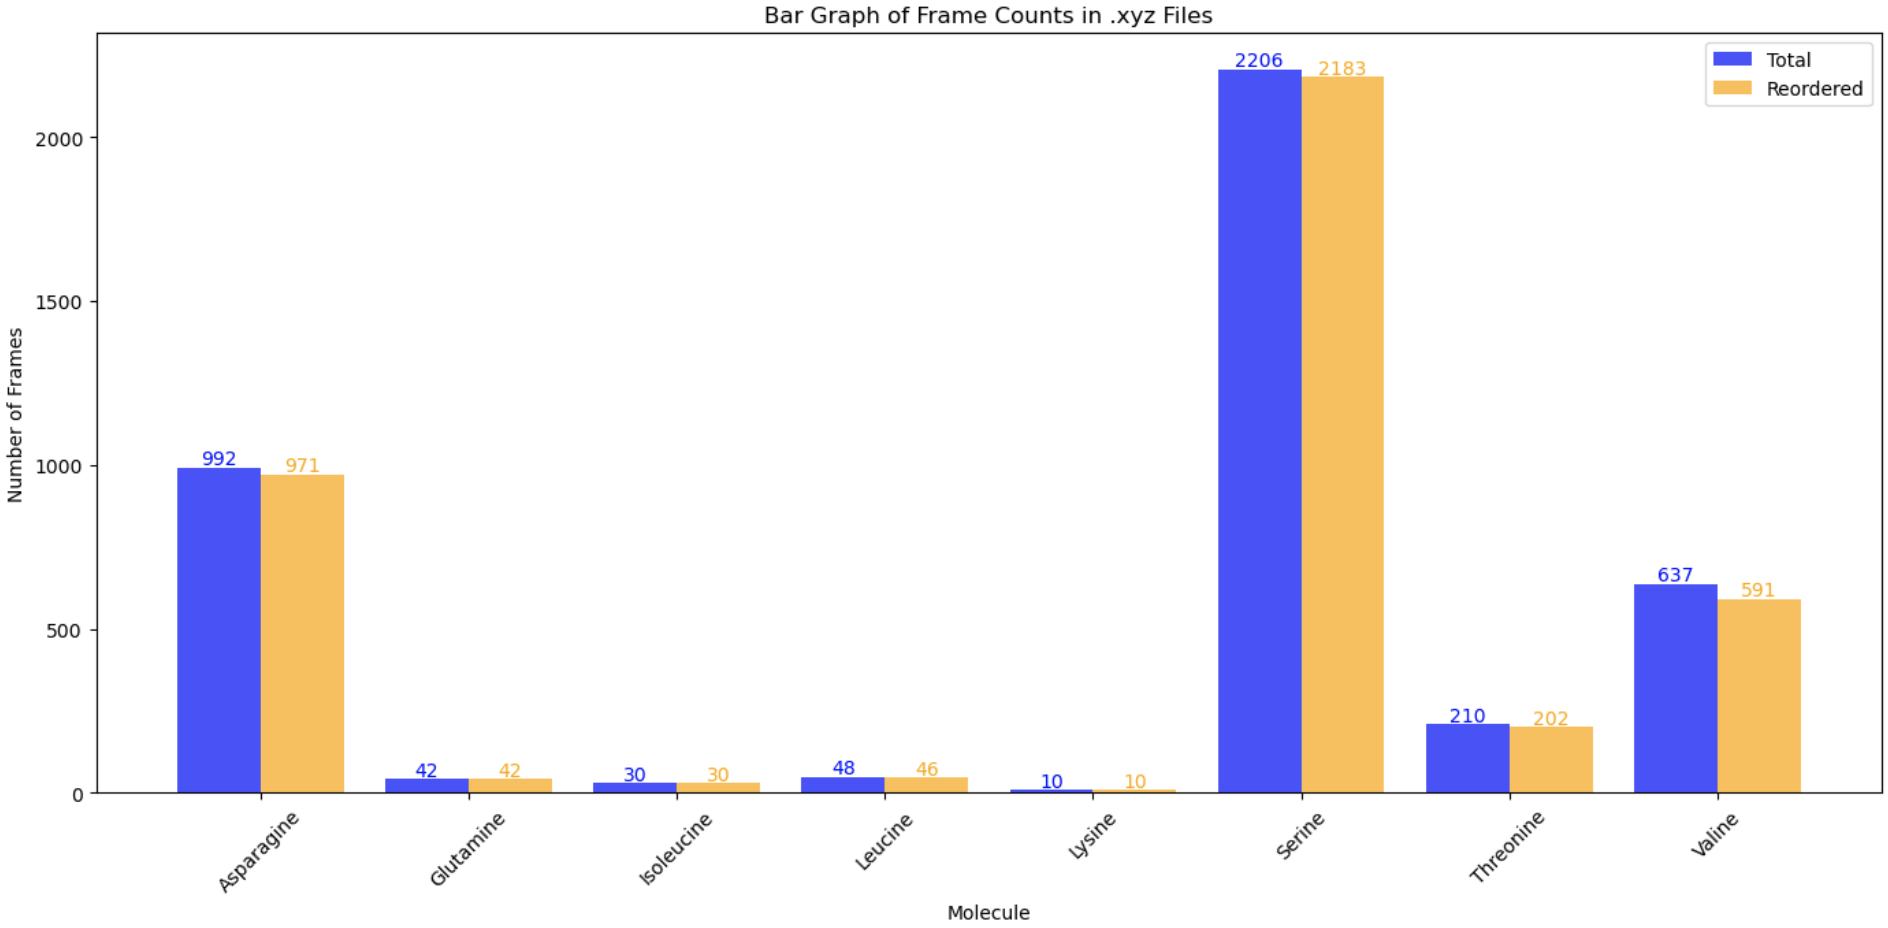
\includegraphics[width=1\linewidth]{Images/early_earth/remake_graph_matching.png}
    \caption[Molecules identified incorrectly in the initial search]{Molecule counts (excluding glycine and alanine) before and after correcting the graph-matching algorithm to account for the proper configuration.}
    \label{fig:graph_matching}
\end{figure}{}

With the corrected graph-matching procedure in place, the identification of alanine molecules in the simulation is now more reliable, allowing for a detailed analysis of their structural properties. 

\begin{figure}[!ht]
    \centering
    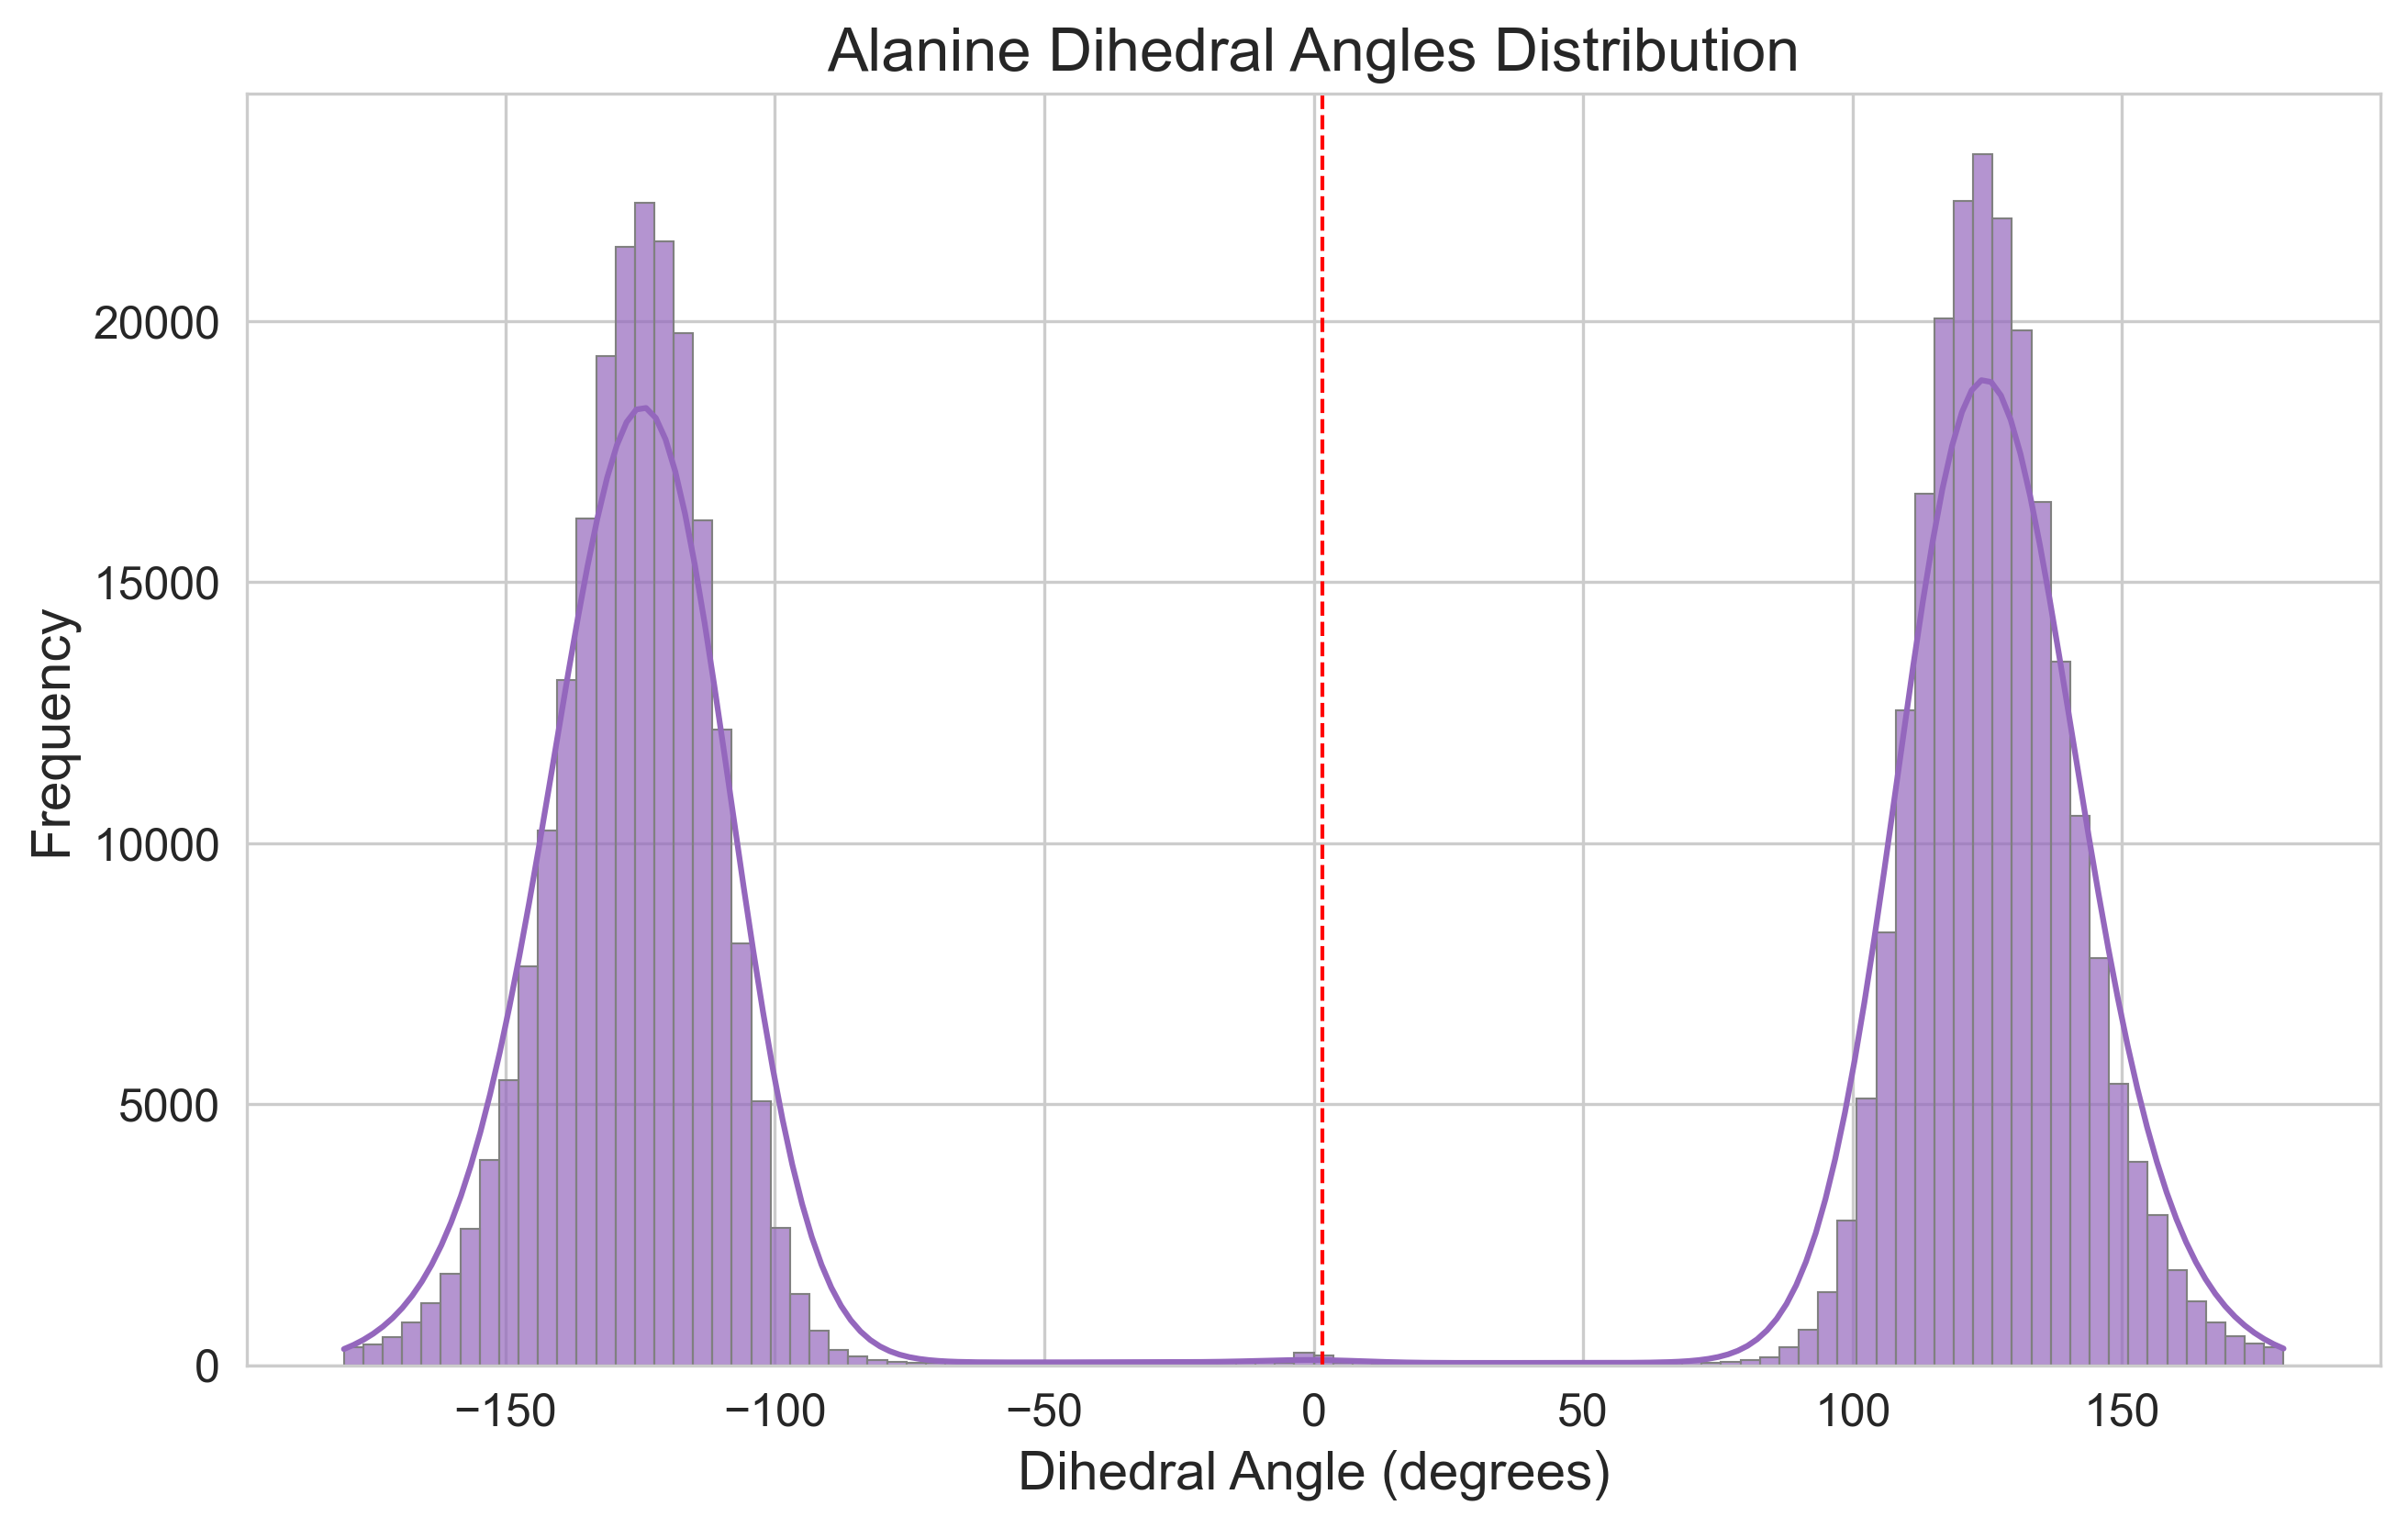
\includegraphics[width=1\linewidth]{Images/alanine_dihedral/dihedral_angles_distribution.png}
    \caption[Distribution of synthesized alanine dihedral angles]{Distribution of dihedral angles in alanine molecules synthesized in the early earth simulation run. Structures obtained from the initial graph search, post-processed with refined graph matching. All molecules fall within the expected range of dihedral angles, centered at $\pm$125$^\circ$.}
    \label{fig:ala_dihedral}
\end{figure}

From the approximately 500,000 alanine molecules synthesized in the Early Earth hero run, dihedral angles were measured to assess conformational distributions. As shown in Figure \ref{fig:ala_dihedral}, the dihedral angles cluster around $\pm$125$^\circ$, consistent with expected alanine geometries. This analysis confirms that the molecular structures identified through the refined graph search not only match the expected connectivity patterns but also exhibit realistic conformational behavior, further validating the accuracy of the updated graph-matching approach.

\subsection{Parallelization}
\label{subsec:molfind_parallelization}

To efficiently process the vast amounts of molecular data generated in the Early Earth simulation, MolFind leverages GPU-accelerated computing through the RAPIDS ecosystem, specifically cuGraph and cuDF, to minimize CPU bottlenecks and perform large-scale graph analysis directly on the GPU. The core of the molecular identification workflow—constructing atomic graphs, finding molecular fragments, and analyzing connectivity—is executed using cuGraph, which provides highly optimized, massively parallel algorithms for graph operations. Instead of iterating through millions of atomic interactions on the CPU, cuGraph’s connected component search rapidly groups atoms into discrete molecular fragments, enabling near-instantaneous classification of structures.

Once fragments are identified, cuDF is used  to store and manipulate molecular descriptors, allowing for rapid filtering, sorting, and aggregation of molecular data while remaining in GPU memory. Unlike traditional CPU-based approaches, which require costly data transfers between RAM and GPU memory, cuDF enables columnar data operations directly within GPU memory, accelerating tasks such as counting molecular occurrences, applying transformations to chemical formulas, and merging results with reference databases. The entire pipeline—from reading molecular dynamics trajectories to identifying molecules and performing statistical analysis—remains within the GPU as much as possible, significantly reducing computation time compared to CPU-bound methods. By using RAPIDS' GPU-native tools, MolFind achieves a scalable approach to analyzing tens of millions of atoms across thousands of trajectory frames, making high-throughput molecular discovery feasible for large-scale simulations.

\section{Restarts -- Quench analysis}
\label{sec:restarts_quench_analysis}

In the Early Earth simulation, 415 selected frames from the 22.8-million-atom system were quenched from 2500 K to 300 K, allowing us to observe how molecular structures stabilize at lower temperatures. The histograms in Figure \ref{fig:ee_quench_hist} compare the distribution of named molecules before and after quenching, highlighting a significant increase in molecular complexity. 

\begin{figure}[!h]
    \centering
    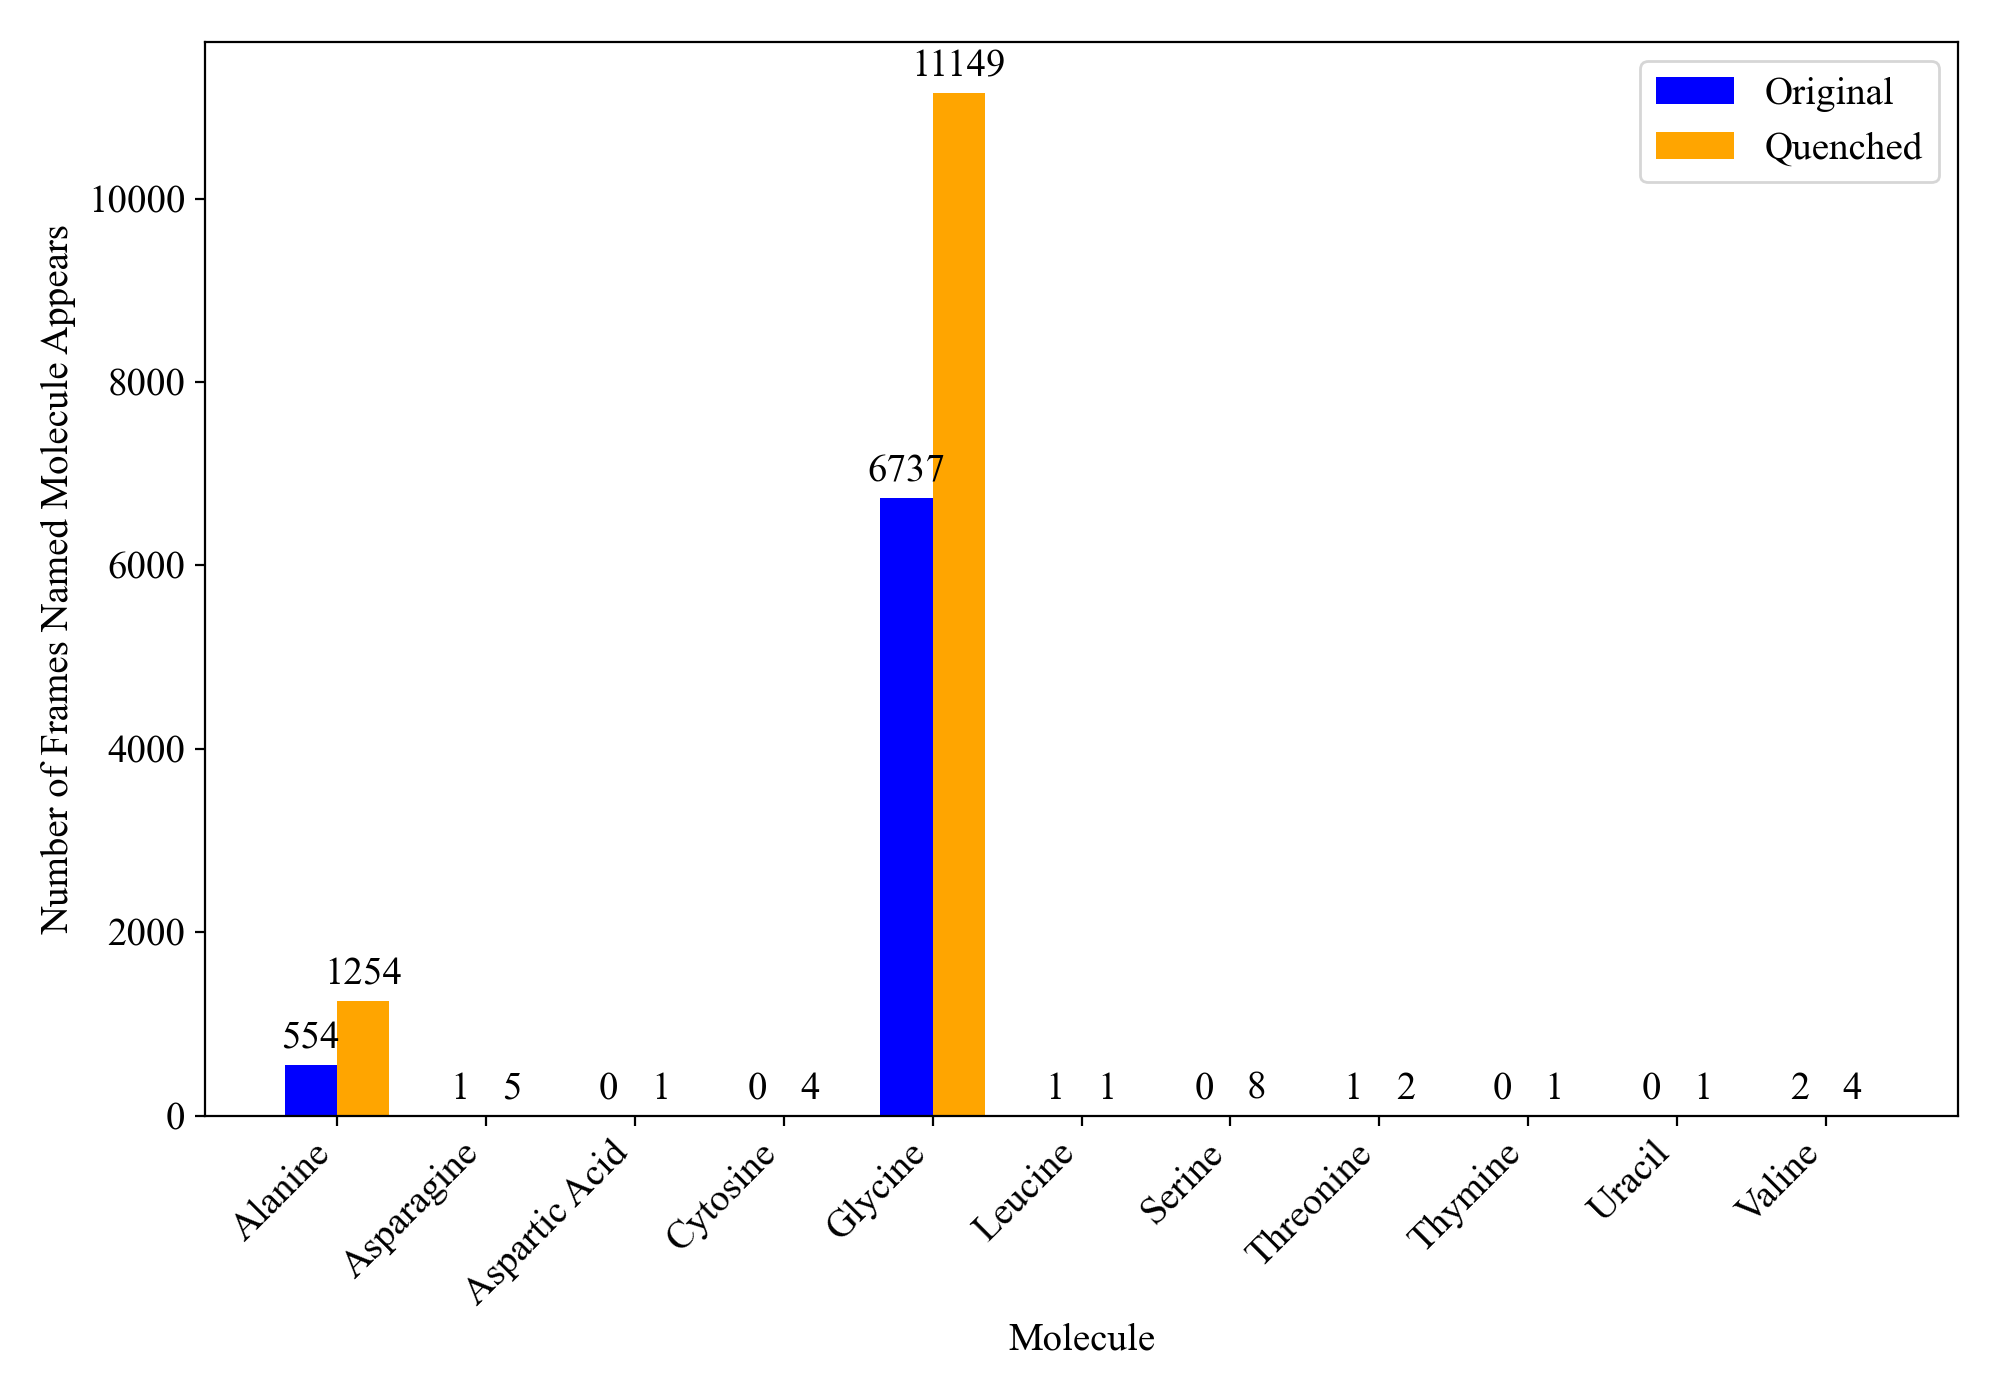
\includegraphics[width=1\linewidth]{Images/early_earth/hist-before-after-quench.png}
    \caption[Histogram: molecules found before and after quenching system]{Histogram of named molecules found before and after quenching 415 selected frames from the 22.8M atom system from 2500 K to 300 K.}
    \label{fig:ee_quench_hist}
\end{figure}

Many smaller fragments coalesced into larger molecules, with a notable rise in carbon-based structures, suggesting that polymerization and oligomerization events occur as the system cools.
This transition is further illustrated in Figure \ref{fig:ee_quench_lineplot}, which tracks the total per-frame count of named molecules before and after the quench. While the total number of individual fragments decreased after cooling, the presence of larger, more chemically diverse molecules increased, indicating that higher-order molecular assembly is favored at lower temperatures.

\begin{figure}[!h]
    \centering
    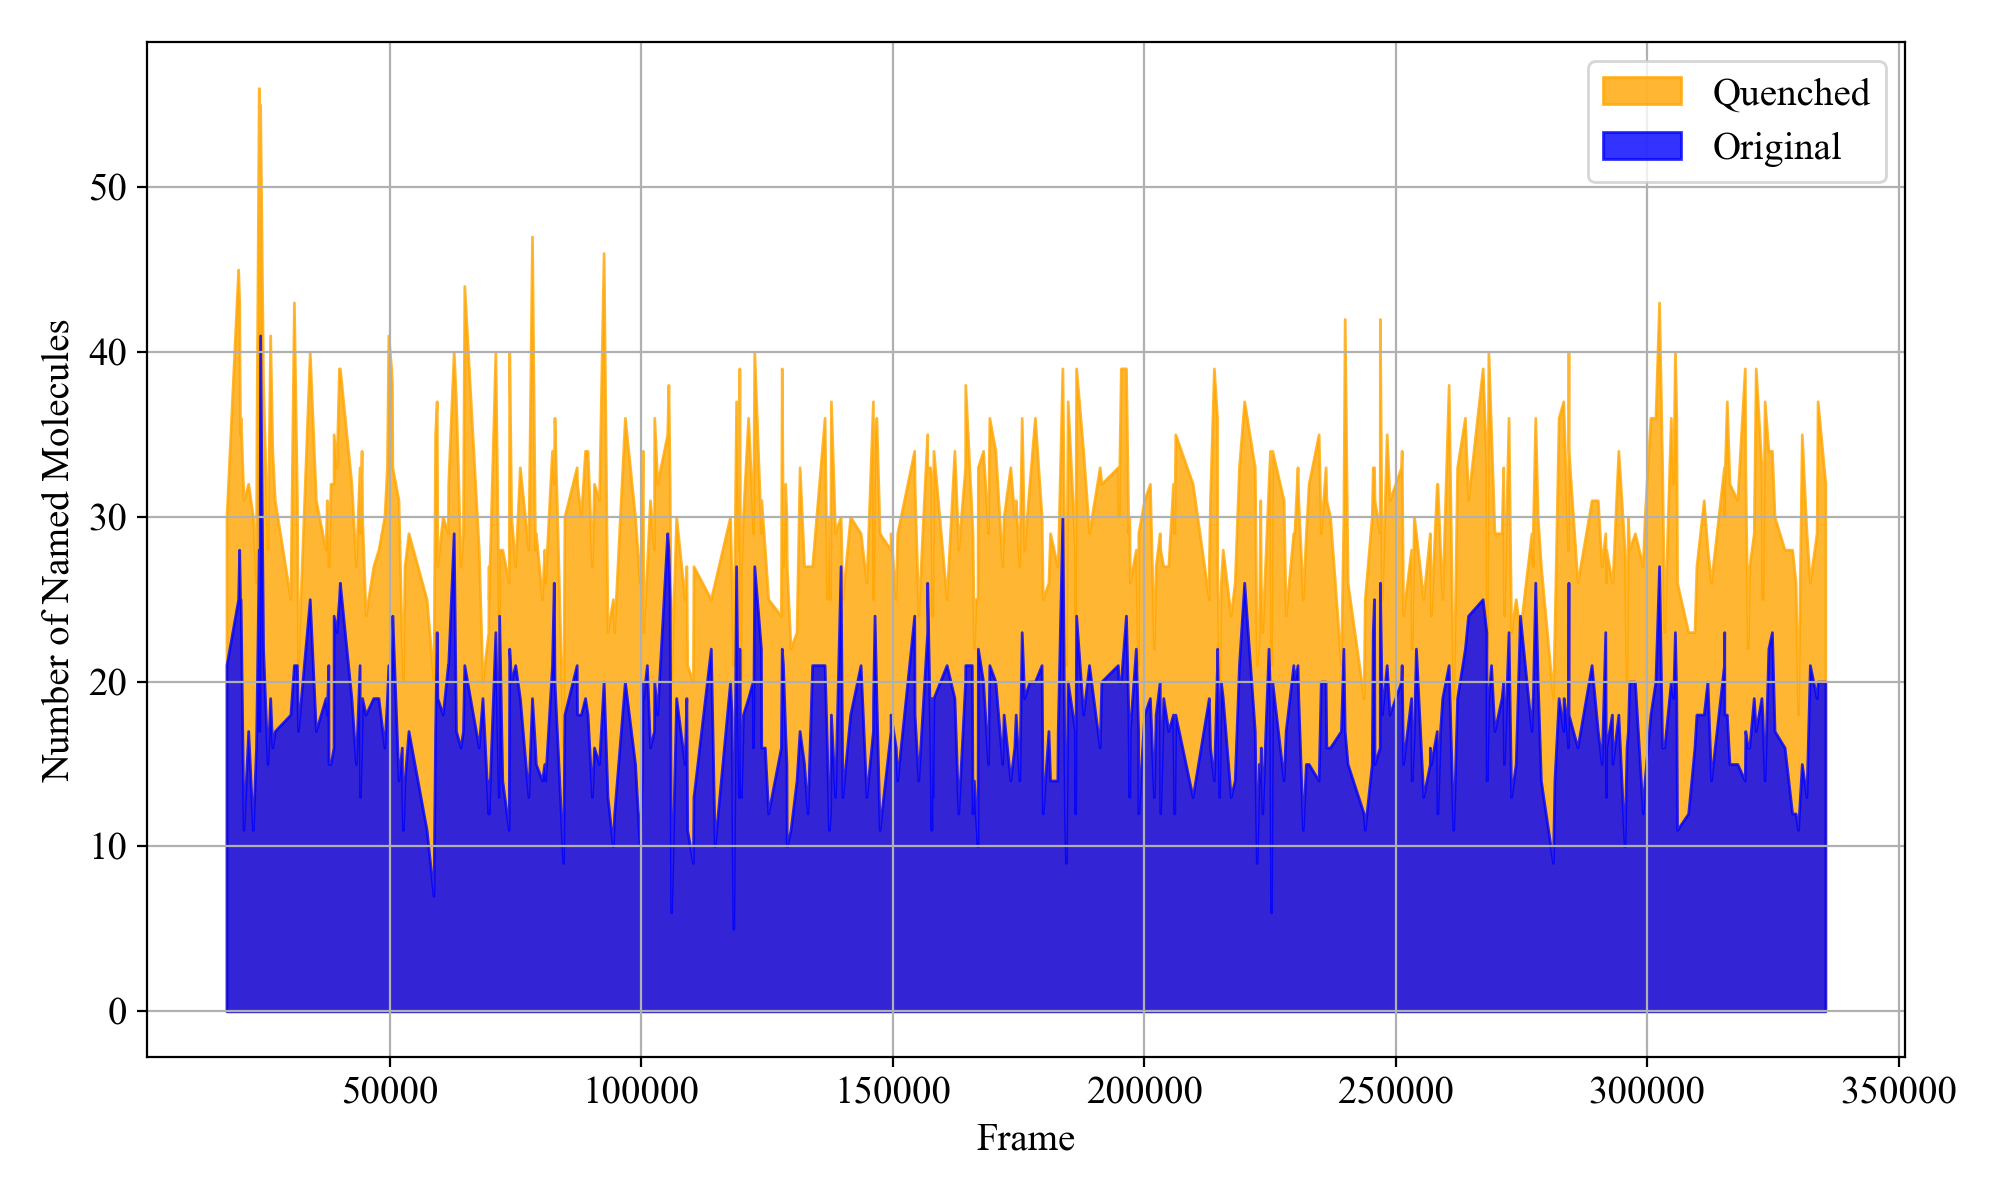
\includegraphics[width=1\linewidth]{Images/early_earth/mol_counts-before-after-quench.png}
    \caption[Line plot: total named molecules found before and after quenching system]{Total per-frame count of named molecules found before and after quenching 415 selected frames from the 22.8M atom system from 2500 K to 300 K.}
    \label{fig:ee_quench_lineplot}
\end{figure}

Prior to quenching, molecular fragments were smaller and more transient, with an average molecule size of 18 atoms per fragment, reflecting the high degree of fragmentation and reactive dynamics at elevated temperatures. However, following the temperature drop, the system exhibited a shift toward larger and more stable molecular species, with the average fragment size increasing to about 30 atoms per molecule in each frame as demonstrated in Figure \ref{fig:ee_quench_violinplot}.

\begin{figure}[!ht]
    \centering
    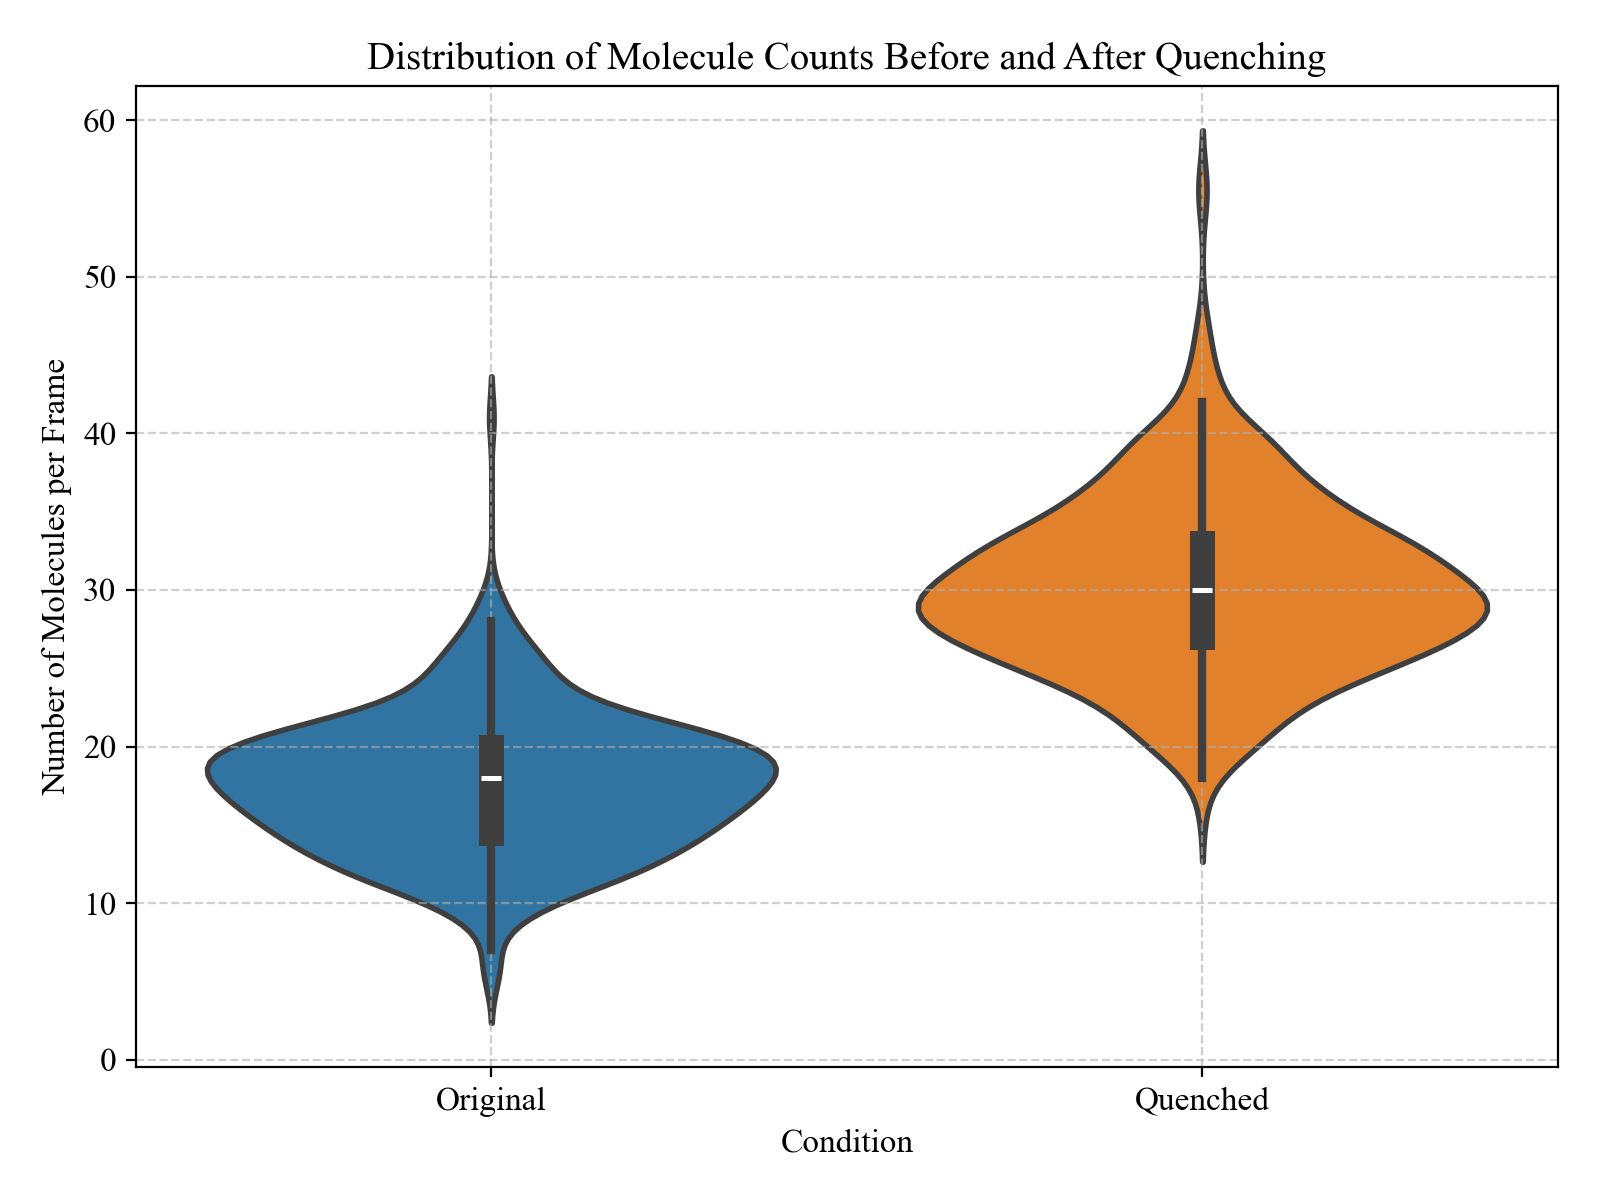
\includegraphics[width=1\linewidth]{Images/early_earth/violinplot-mol_counts-before-after-quench.png}
    \caption[Violin plot: total named molecules found before and after quenching system]{Distribution of per-frame counts of named molecules found before and after quenching 415 selected frames from the 22.8M atom system from 2500 K to 300 K.}
    \label{fig:ee_quench_violinplot}
\end{figure}

This analysis reinforces the idea that thermal history plays a crucial role in the emergence of molecular complexity, with high-temperature conditions promoting fragmentation and chemical diversity, while subsequent cooling allows for the stabilization of more intricate molecular architectures. These findings provide key insights into potential prebiotic chemistry pathways, where transient high-energy environments could generate molecular building blocks that later assemble into more stable organic structures under cooler conditions.

\section{Exploring New Molecular Configurations}
\label{sec:exploring_new_mol_configs}

As mentioned in Subsection \ref{subsec:drawback_config_sampling}, configurational is difficult in the active learning via query by committee used in generating ANI datasets, and as a result new molecular configurations have been sampled from enumeration datasets and other curated chemical datasets.
The ANI-1xnr \cite{ani-1xnr} approach to generating training set data via nanoreactors and other approaches taken in 1xnr paper serves as an inspiration for sampling new configurations from a massive batch of reaction data.


\section{Interpretation of Results}
\label{sec:hero_run_interpretation}

Our initial search targeted 357 molecules of biological relevance, specifically focusing on fundamental building blocks of life. These included the 20 proteinogenic amino acids, all possible dipeptides formed by combinations of these amino acids, the five canonical nucleobases (adenine, guanine, cytosine, thymine, and uracil), simple fatty acids, and other known prebiotic molecules hypothesized to emerge under early Earth conditions. This set was chosen to reflect both experimentally observed prebiotic chemistry, such as the Miller-Urey experiment, and biologically significant molecules that play a role in protein synthesis, nucleotide formation, and metabolic pathways.

From this initial search, using this limited but biologically relevant list, we identified nearly 6 million occurrences of named biomolecules throughout the simulation---listed in Table \ref{tab:inital_molfind_counts}. 

\begin{table}[hb]
    \centering
    \begin{tabularx}{3in}{Xr}
        \toprule
        Molecule name & Molecules identified \\
        \midrule
        Glycine & 5,297,484 \\
        Alanine & 445,342 \\
        Serine & 2,183 \\
        Asparagine & 971 \\
        Valine & 591 \\
        Aspartic Acid & 439 \\
        Uracil & 414 \\
        Cytosine & 227 \\
        Threonine & 202 \\
        Caprylic acid & 137 \\
        Leucine & 46 \\
        Glutamine & 42 \\
        Glutamic Acid & 37 \\
        Isoleucine & 30 \\
        GlycylGlycine & 14 \\
        Lysine & 10 \\
        Thymine & 9 \\
        \bottomrule
    \end{tabularx}
    \caption[Initial Early Earth molfind search]{The molecules identified in the initial analysis of the Hero Run data.}
    \label{tab:inital_molfind_counts}
\end{table}

The vast majority of these identifications were glycine, the simplest amino acid, which appeared over 5.2 million times. This high frequency aligns with glycine’s known prebiotic abundance and its formation in numerous laboratory simulations of early Earth conditions. Alanine, another small and structurally simple amino acid, was the second most commonly detected species, appearing in over 445,000 instances. Beyond these, we identified additional amino acids—including serine, asparagine, valine, and aspartic acid—as well as nucleobases such as uracil and cytosine, which are essential components of RNA.

A particularly interesting result was the identification of dipeptides, including glycylglycine, which was detected 14 times in the dataset. The presence of peptide bonds suggests that polymerization reactions were occurring within the simulation, possibly facilitated by the high-temperature conditions and reactive intermediates. Additionally, we detected caprylic acid, a medium-chain fatty acid, which may indicate the formation of simple lipid-like molecules under these conditions. While many larger amino acids, such as leucine, glutamine, and lysine, were detected in only a handful of instances, their presence supports the hypothesis that molecular complexity can emerge from simple precursors given the right conditions.

This initial analysis represents a conservative lower bound on molecular diversity within the simulation, as it only considers molecules from our predefined list. As subsequent searches expand beyond this initial set to include all possible molecular structures that obey valence rules, we anticipate uncovering an even greater variety of prebiotic molecules, shedding further light on the chemical pathways that may have led to life’s molecular precursors.

\section{Expanding the Search}
\label{sec:expanding_the_search}

Following the initial search, efforts have been made to expand the molecular identification process beyond the predefined set of 357 biomolecules. By leveraging the graph-based molecular search framework, we aim to systematically identify all possible molecular structures that form within the simulation while adhering to chemical valence rules. This expansion is motivated by both experimental and astronomical evidence suggesting that early Earth conditions and extraterrestrial bodies may have harbored a much broader range of prebiotic molecules than previously considered.

Recent studies have demonstrated that protocell-like structures and prebiotic compounds can form simultaneously under plausible early Earth atmospheric conditions, supporting the idea that a diverse chemical inventory existed in prebiotic environments \cite{prebiotic_compounds_EE_atmosphere}. Similarly, analysis of asteroid samples has revealed an abundance of ammonia and nitrogen-rich organic matter, further suggesting that prebiotic molecules were not only synthesized on Earth but may have also been delivered via extraterrestrial sources \cite{astroid_sample}. These findings reinforce the importance of broadening our molecular search beyond canonical biological molecules to include a more diverse range of heterocyclic compounds, reactive intermediates, and non-proteinogenic amino acids that may have played a role in prebiotic chemistry.

To address this, we are refining molecular graph searching algorithms to dynamically detect and classify novel molecular species based on their connectivity and bonding patterns. By allowing the search space to grow beyond known biological molecules, we can systematically explore the chemical landscape of early Earth, uncovering potential precursors to metabolic and structural biomolecules that may have contributed to the origins of life.